\documentclass{beamer}
% \usepackage{lmodern}
%=====================================================================
% Color definition
\definecolor{jvagreen}{RGB}{0,104,	139}
\definecolor{jvagold}{RGB}{255, 255, 255}
\setbeamercolor{section in head/foot}{fg = jvagold, bg = jvagreen}
\usepackage{graphicx}
\usepackage{mathtools}
\usepackage{picture}
\usepackage{amsmath}
\usepackage{multimedia}
\DeclareMathOperator{\Tr}{Tr}
%\graphicspath{{../}}
\setbeameroption{show notes}
\usepackage{multicol}
\usepackage[compatibility=false]{caption}
\usepackage{caption}
\usepackage{subcaption} % To use subfigures with subcaptions
\usepackage{textpos}

\captionsetup[subfigure]{labelformat=empty}
\renewcommand{\figurename}{}
\usepackage[labelsep=endash]{caption}

\usepackage{wrapfig}
\definecolor{light-gray}{gray}{0.95}
\usepackage{tcolorbox}

\newcommand{\phim}{\mathbf{\phi}}
\newcommand{\X}{\mathbf{X}}
\newcommand{\x}{\mathbf{x}}
\newcommand{\Y}{\mathbf{Y}}
\newcommand{\y}{\mathbf{y}}
\newcommand{\w}{\mathbf{w}}
\newcommand{\Z}{\mathbf{Z}}
\newcommand{\z}{\mathbf{z}}
\newcommand{\h}{\mathbf{h}}
\newcommand{\dd}{\: \mathrm{d}}
\newcommand{\B}{\mathbf{B}}
\newcommand{\F}{\mathbf{F}}
\newcommand{\bb}{\mathbf{b}}
\newcommand{\vect}[1]{\mathbf{#1}}

\usebackgroundtemplate
{
    
\includegraphics[width=\paperwidth,height=\paperheight]{img/blank.jpg}%
}
\beamertemplatenavigationsymbolsempty

%=====================================================================
% Templates - headline, frametitle

\makeatletter
% Komprimiert die miniframe Kreise auf eine Linie
\beamer@compresstrue
\makeatother

% Definiert die headline
\setbeamertemplate{headline}
{ 
%\includegraphics[width=\paperwidth]{pic} % test logo
\begin{beamercolorbox}[wd=\paperwidth,right]{section in head/foot}
    \rule{\paperwidth}{1pt}
    %Vertikaler Abstand
    \vskip20pt
    %Fügt die Standard-Navi ein (miniframes)
    %\insertnavigation{\paperwidth}
    \vskip8pt
    %\rule{\paperwidth}{0.5pt}
    %\vskip25.5pt % same height of the example provided, but IMHO is too much
    \rule{\paperwidth}{1pt}
\end{beamercolorbox} 
}
\setbeamertemplate{footline}
{ 
%\includegraphics[width=\paperwidth]{pic} % test logo
\begin{beamercolorbox}[wd=\paperwidth,right]{section in head/foot}
    \rule{\paperwidth}{1pt}
    %Vertikaler Abstand
    \vskip10pt
    %Fügt die Standard-Navi ein (miniframes)
    \insertnavigation{\paperwidth}
    \vskip8pt
    \rule{\paperwidth}{0.5pt}
    %\vskip25.5pt % same height of the example provided, but IMHO is too much
    %\rule{\paperwidth}{1pt}
\end{beamercolorbox} 
}

% definition of the frametitle
\setbeamertemplate{frametitle}
{
\vskip-24pt % to shift up the frametitle
\hbox{ 
 \begin{beamercolorbox}[wd=.0675\textwidth]{} % left shift
 \end{beamercolorbox} 
 \begin{beamercolorbox}[sep=4pt]{section in head/foot}
 \insertframetitle
 \end{beamercolorbox} 
 }
}

\mode<presentation>
{
    \setbeamertemplate{itemize item}[circle]
    \setbeamercolor{itemize item}{fg = jvagreen}
    \setbeamertemplate{itemize subitem}[circle]
    \setbeamercolor{itemize subitem}{fg = jvagreen}
}

\renewcommand\footnoterule{}

\AtBeginSection[]
{
  \begin{frame}<beamer>
    \frametitle{Outline}
    \tableofcontents[currentsection]
  \end{frame}
}

%\logo{\includegraphics[height=0.6cm]{img/cde_basic_green}}
%\let\oldequation=\equation
%\let\endoldequation=\endequation
%\renewenvironment{equation}{\vspace{1cm}\begin{oldequation}}{\end{oldequation}\vspace{15mm}}

\begin{document}

\addtobeamertemplate{frametitle}{}{%
\begin{textblock*}{100mm}(-0.9cm,-0.6cm)

\includegraphics[height=0.5cm,width=1.5cm]{img/uob-logo-white-transparent}
\end{textblock*}
\begin{textblock*}{100mm}(0.97\textwidth,-0.6cm)

\includegraphics[height=0.5cm,width=1cm]{img/cde_tag_white}
\end{textblock*}
}

\title[Performance-driven Facial Animation]{
  Performance-driven Facial Animation}

% Optional: a subtitle to be dispalyed on the title slide
% \subtitle{Show where you're from}
% \subtitle{Presented by: Ieva Kazlauskaite}
% The author(s) of the presentation:
%  - again first a short version to be displayed at the bottom;
%  - next the full list of authors, which may include contact information;
\author[Garoe Dorta Perez, Ieva Kazlauskaite, Richard Shaw]{
   Garoe Dorta Perez, Ieva Kazlauskaite, Richard Shaw } 


% The institute:
%  - to start the name of the university as displayed on the top of each slide
%    this can be adjusted such that you can also create a Dutch version
%  - next the institute information as displayed on the title slide
\institute[University of Bath]{
University of Bath \\
Centre For Digital Entertainment
}

% Add a date and possibly the name of the event to the slides
%  - again first a short version to be shown at the bottom of each slide
%  - second the full date and event name for the title slide

\date{27 May 2015}

% TITLE PAGE
\begin{frame}[plain]
  \titlepage
\end{frame}

%\section{Overview}
% CONTENT PAGE
%\begin{frame}
%  \frametitle{Overview}
%  \tableofcontents
%\end{frame}

%----------------------------------------------------------------------
\section{Data Capture and 3D Reconstruction}
\begin{frame}{Data Capture}

\begin{itemize}
\setlength\itemsep{0.5em}
\item Performance capture using two DSLR cameras in stereo.
\item Video recorded at 60fps with resolution $640 \times 480$ pixels.
\item Video streams synchronised using audio signals.
\end{itemize}

\begin{center}
\begin{figure}
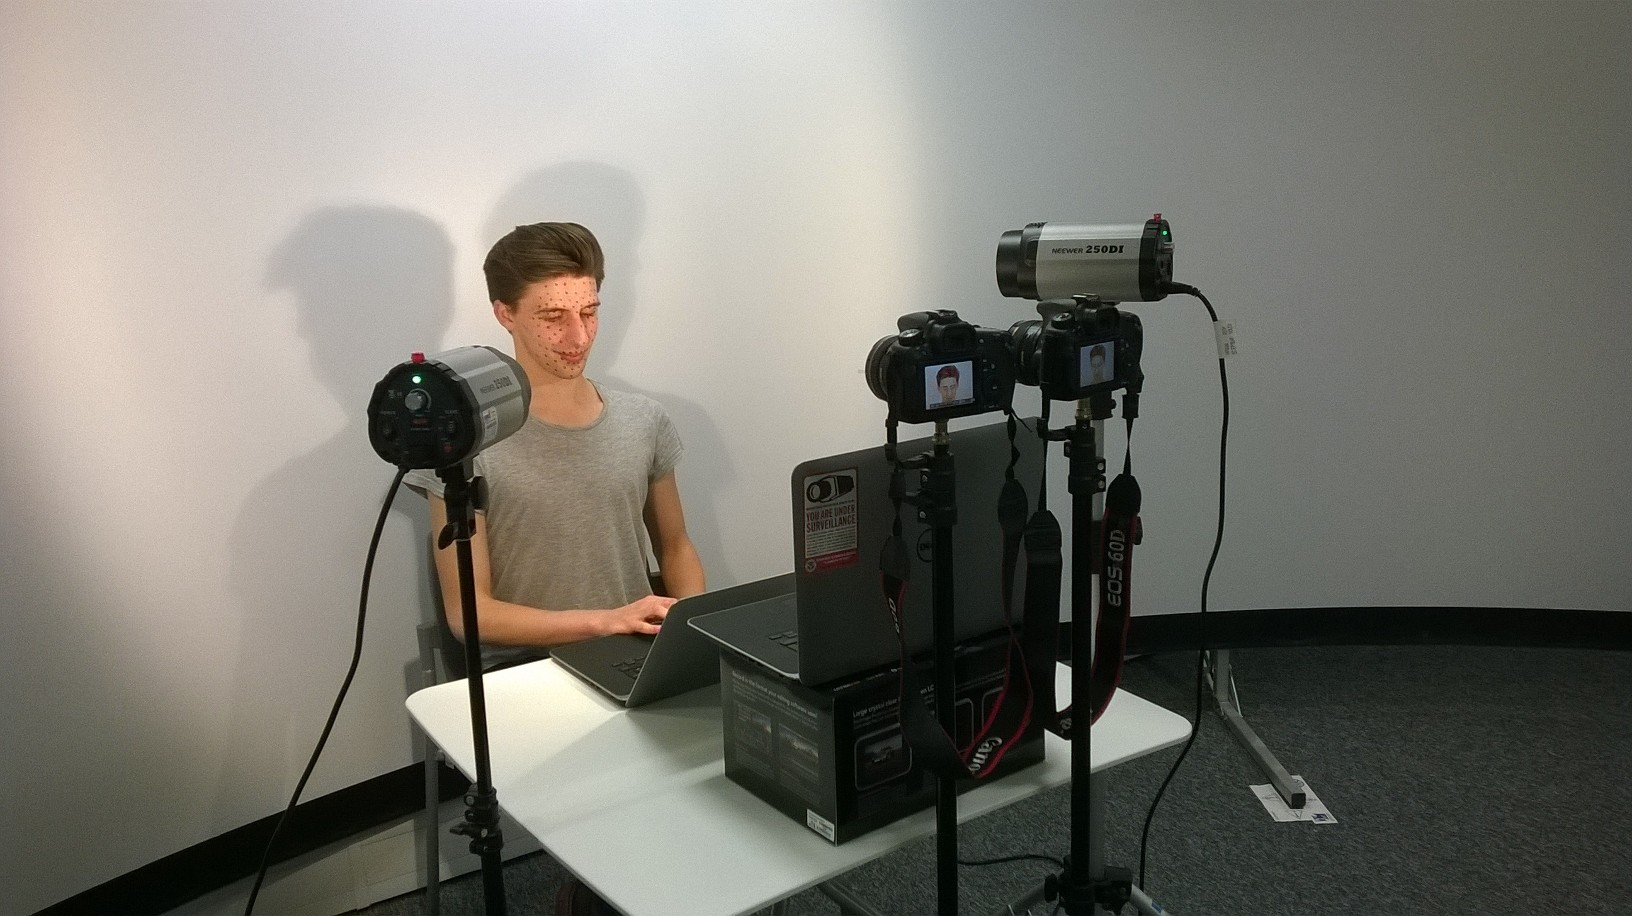
\includegraphics[width=0.7\textwidth]{img/setup1}
\caption{\tiny{The data capture session using two DSLR cameras in stereo.}}
\end{figure}
\end{center}

\end{frame}



\begin{frame}{Face Markers}

\begin{itemize}
\setlength\itemsep{0.5em}
\item Markers are drawn onto the actor's face to track the facial performance.
\end{itemize}

\begin{center}
\begin{figure}
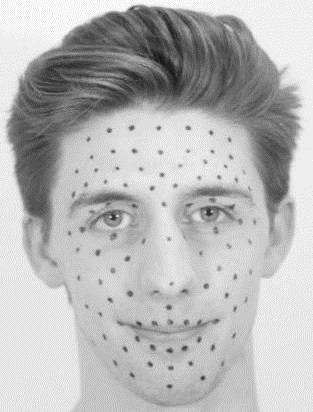
\includegraphics[width=0.35\textwidth]{img/facemarkers} ~
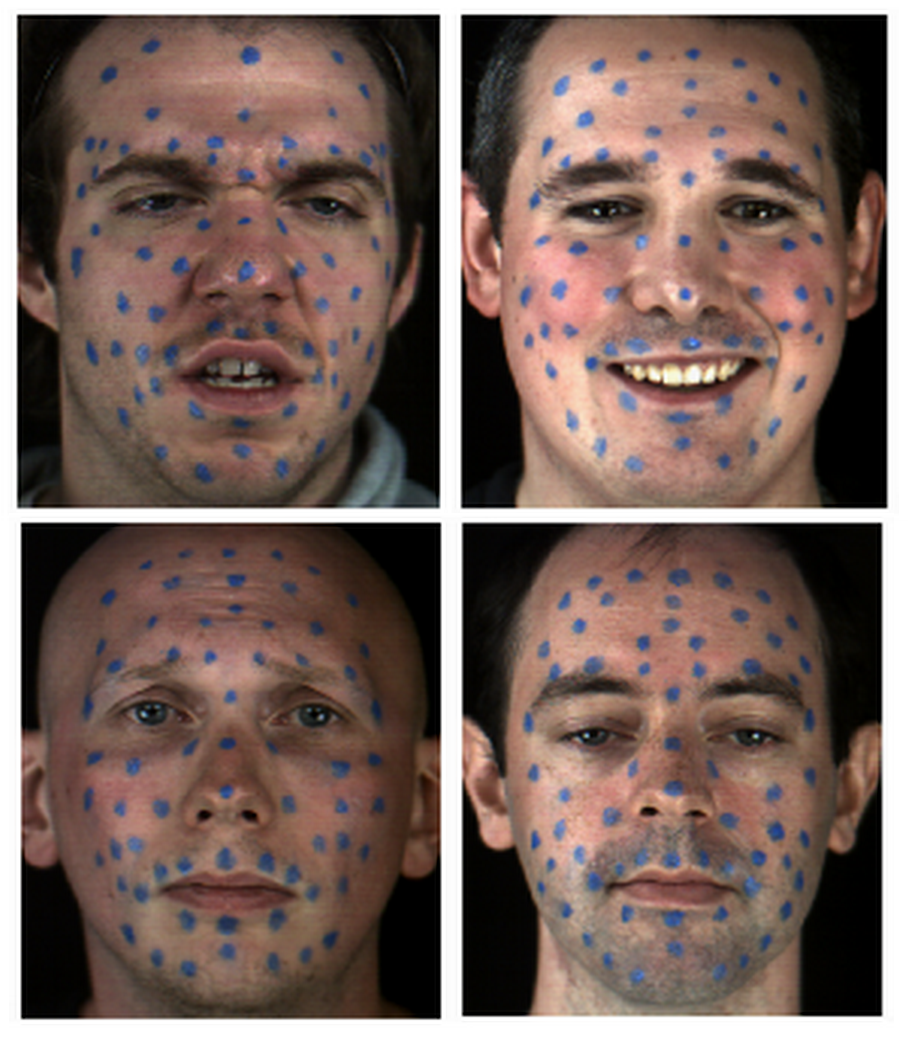
\includegraphics[width=0.4\textwidth]{img/surreydata}
\caption{\tiny{Marker positions were roughly based on the Surrey Audio-Visual Expressed Emotion (SAVEE) Database.}}
\end{figure}
\end{center}

\end{frame}



\begin{frame}{Stereo Calibration}

\begin{itemize}
\setlength\itemsep{0.5em}
\item A checkerboard pattern used to calibrate stereo camera setup.
\item Obtain the cameras' intrinsic and external parameters.
\item Compute the projection matrices and fundamental matrix.
\end{itemize}

\begin{center}
\begin{figure}
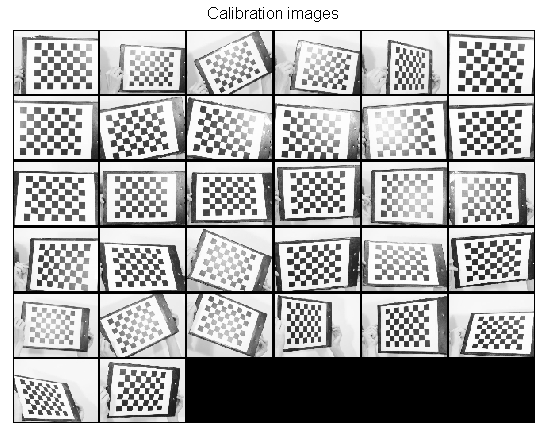
\includegraphics[width=0.4\textwidth]{img/checkerboard} ~
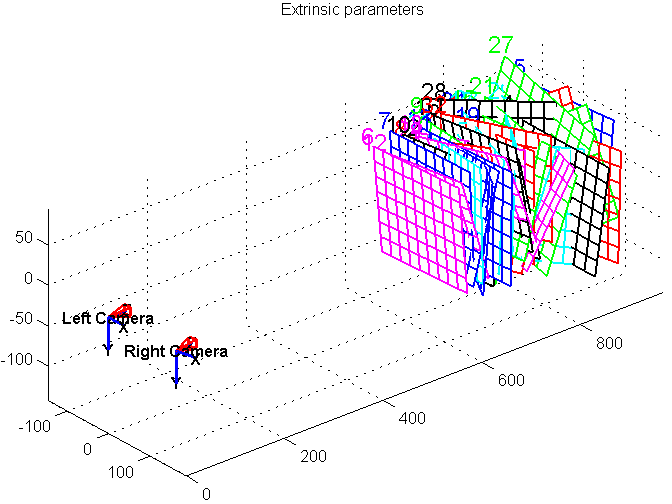
\includegraphics[width=0.42\textwidth]{img/calib}
\caption{\tiny{The stereo cameras were calibrated using a checkerboard pattern.}}
\end{figure}
\end{center}

\end{frame}



\begin{frame}{Stereo Rectification}

\begin{itemize}
\setlength\itemsep{0.5em}
\item Using the camera parameters we rectify each stereo pair for a captured image sequence.
\item Corresponding epipolar lines lie on the same pixel rows.
\item Reduces correspondence problem to a 1D search.
\end{itemize}

\begin{center}
\begin{figure}
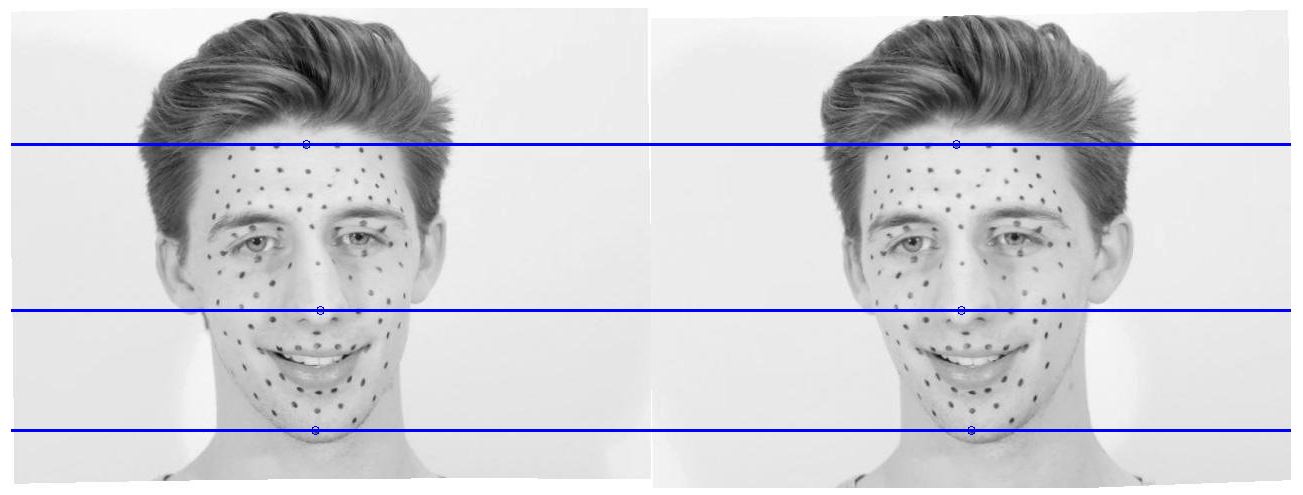
\includegraphics[width=0.8\textwidth]{img/epipolarlines}
\caption{\tiny{Each frame of an image sequence is stereo rectified.}}
\end{figure}
\end{center}

\end{frame}



\begin{frame}{Initial Marker Detection}

\begin{itemize}
\setlength\itemsep{0.5em}
\item Face markers are detected by computing SIFT features in the left image of the first frame.
\item Wrongly detected pixels can be removed and additional points included interactively.
\end{itemize}

\begin{center}
\begin{figure}
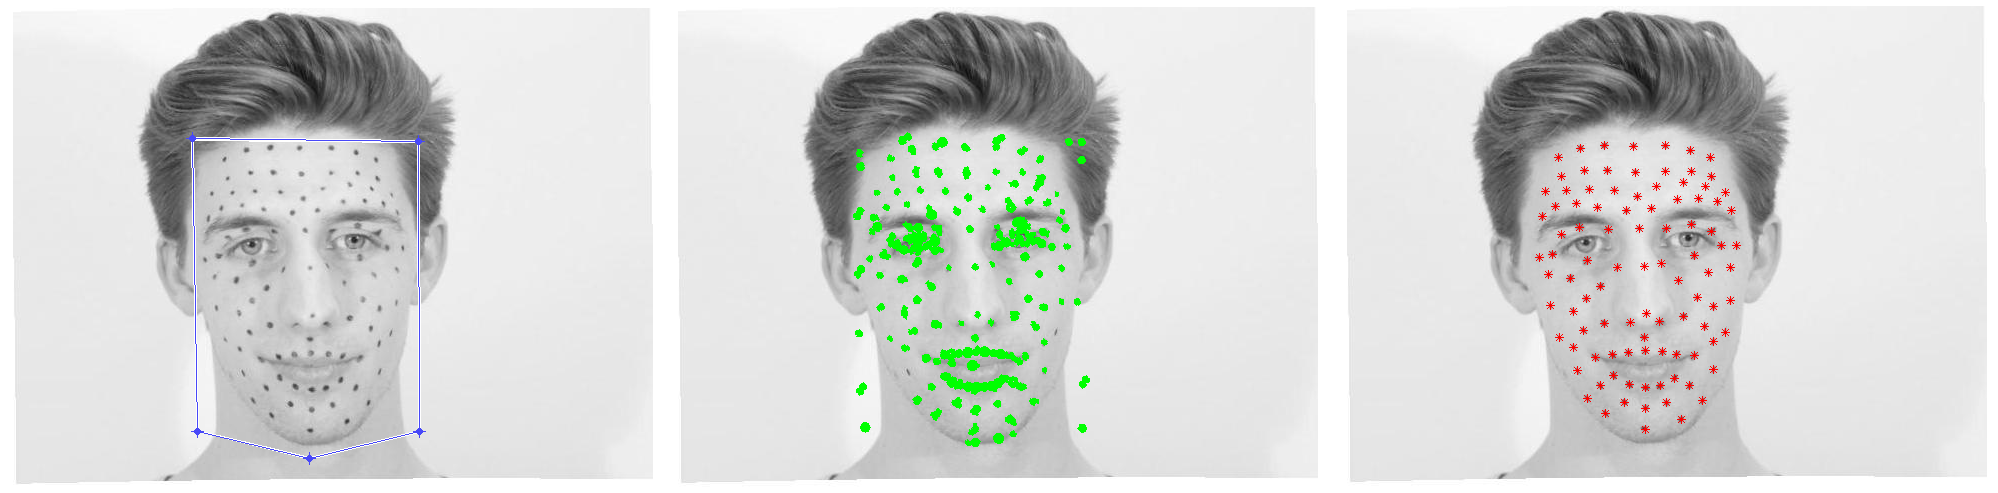
\includegraphics[width=1.0\textwidth]{img/detection}
\caption{\tiny{Markers on the face are detected using SIFT features.}}
\end{figure}
\end{center}

\end{frame}



\begin{frame}{Feature Matching}

\begin{itemize}
\setlength\itemsep{0.5em}
\item Corresponding markers in the right image are found by searching along the corresponding epipolar lines.
\item Matching features are found by computing the normalised cross-correlation for image patches around each feature point.
\end{itemize}

\begin{center}
\begin{figure}
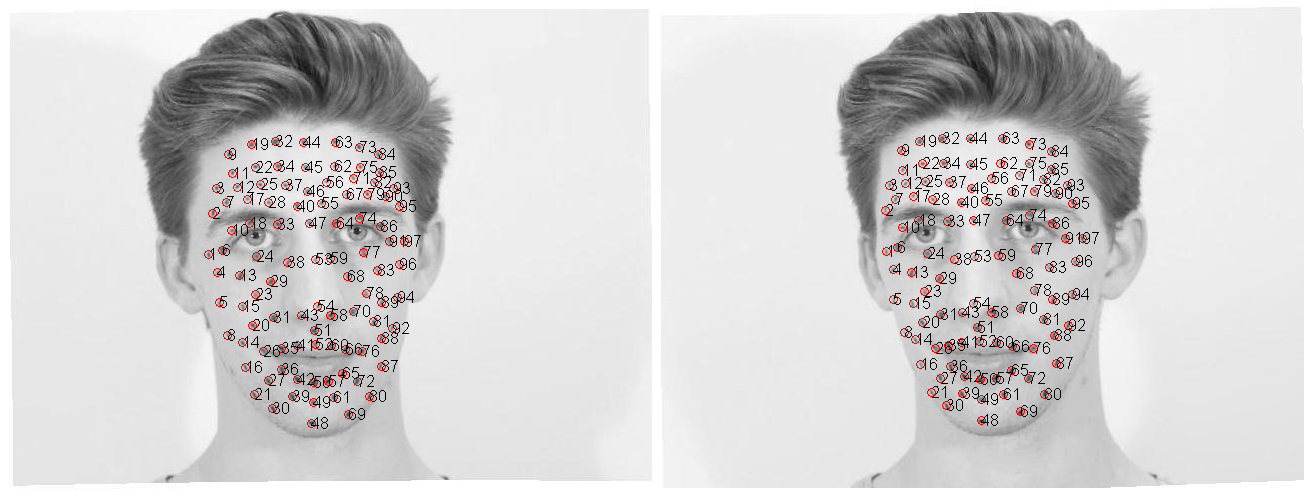
\includegraphics[width=1.0\textwidth]{img/matching}
\caption{\tiny{Corresponding markers are found in the right image.}}
\end{figure}
\end{center}

\end{frame}



\begin{frame}{Marker Tracking}

\begin{itemize}
\setlength\itemsep{0.5em}
\item We track the face markers throughout the entire image sequence using the KLT tracking algorithm.
\end{itemize}

\begin{center}
\begin{figure}
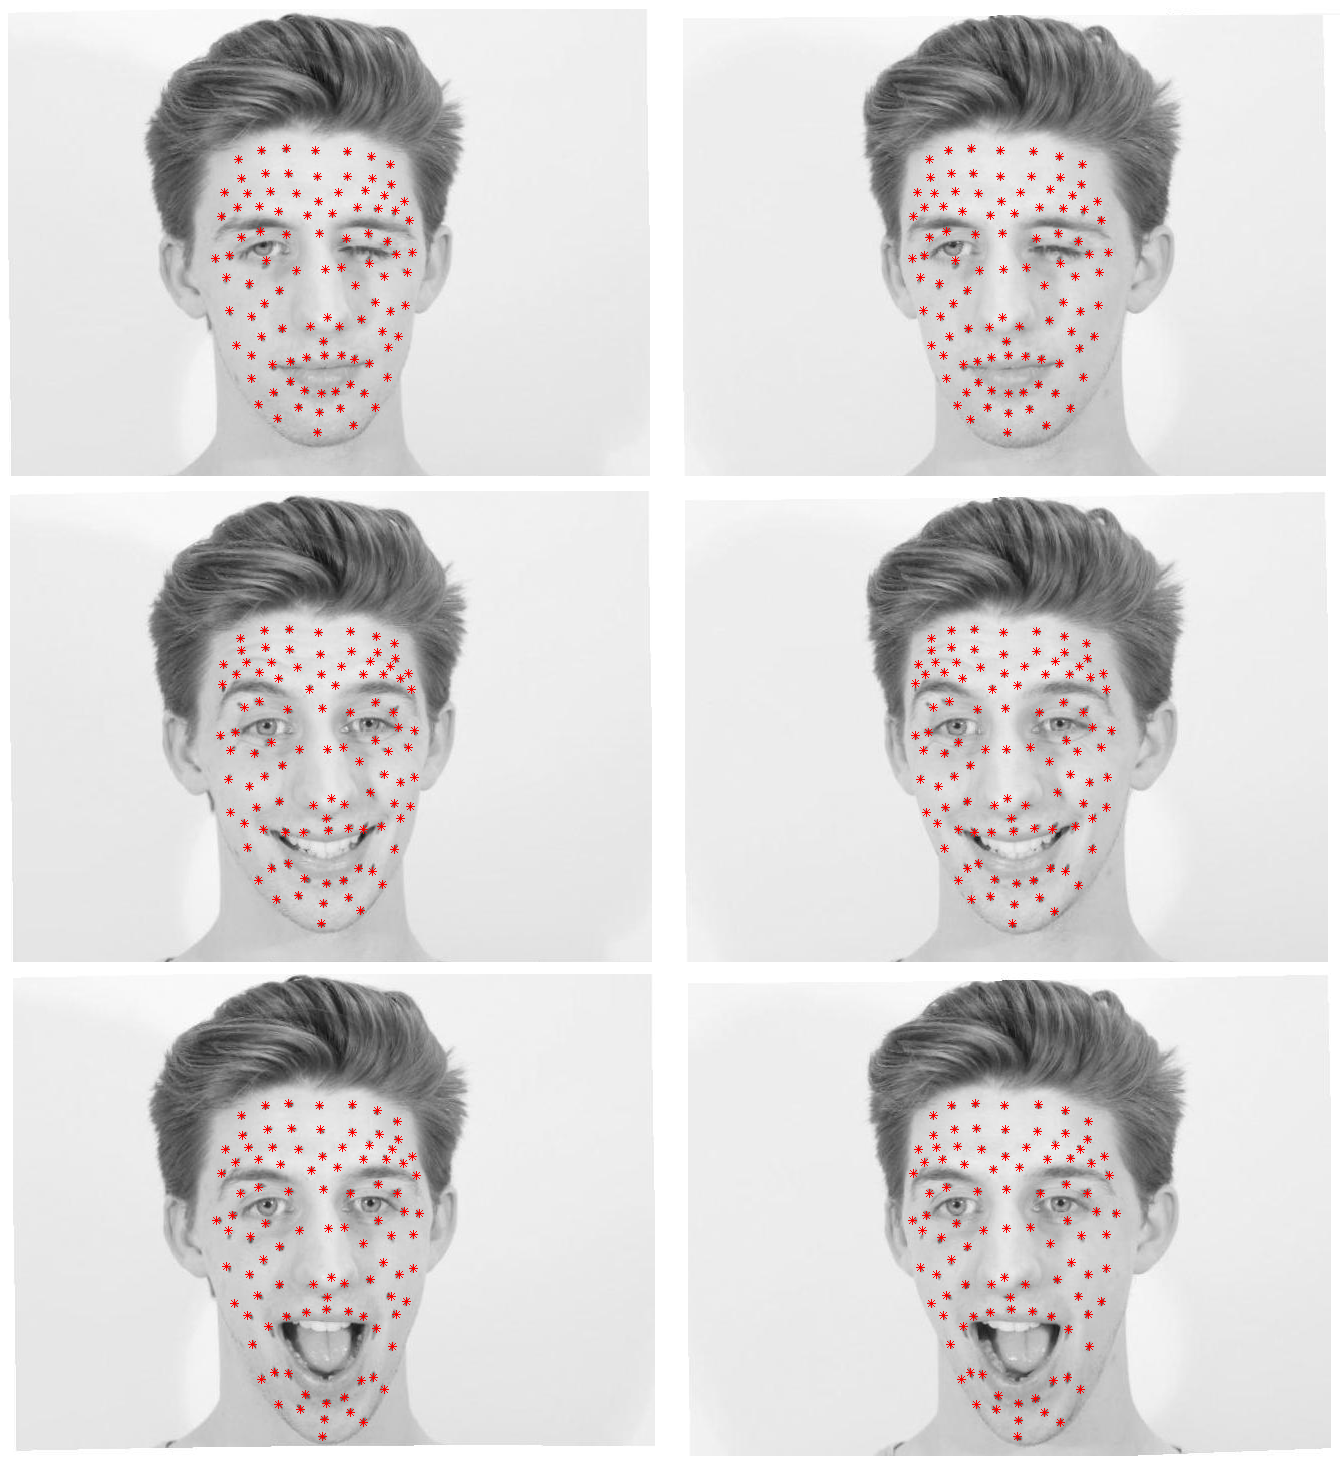
\includegraphics[width=0.5\textwidth]{img/tracking}
\end{figure}
\end{center}

\end{frame}




\begin{frame}{Sparse 3D Reconstruction}

\begin{itemize}
\setlength\itemsep{0.5em}
\item Using the known camera projection matrices, we compute a sparse 3D reconstruction by triangulating.
\end{itemize}

\begin{center}
\begin{figure}
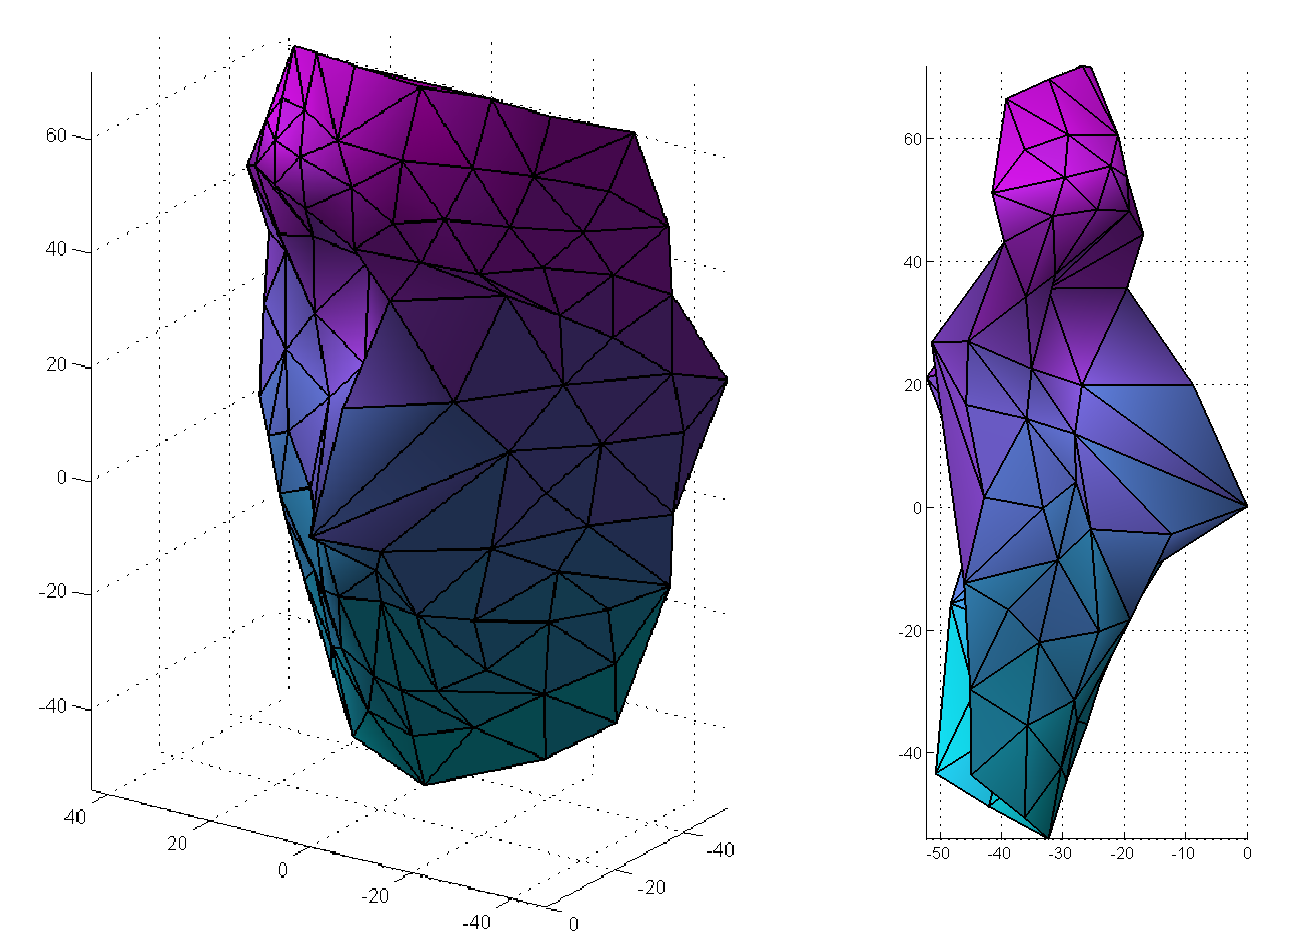
\includegraphics[width=0.6\textwidth]{img/face}
\caption{\tiny{The 3D reconstruction of the neutral expression.}}
\end{figure}
\end{center}

\end{frame}



\begin{frame}{Sparse Sequence Reconstruction}

\begin{itemize}
\setlength\itemsep{0.5em}
\item Using the known camera projection matrices, we compute a sparse 3D reconstruction for every frame.
\end{itemize}

\begin{center}
\begin{figure}
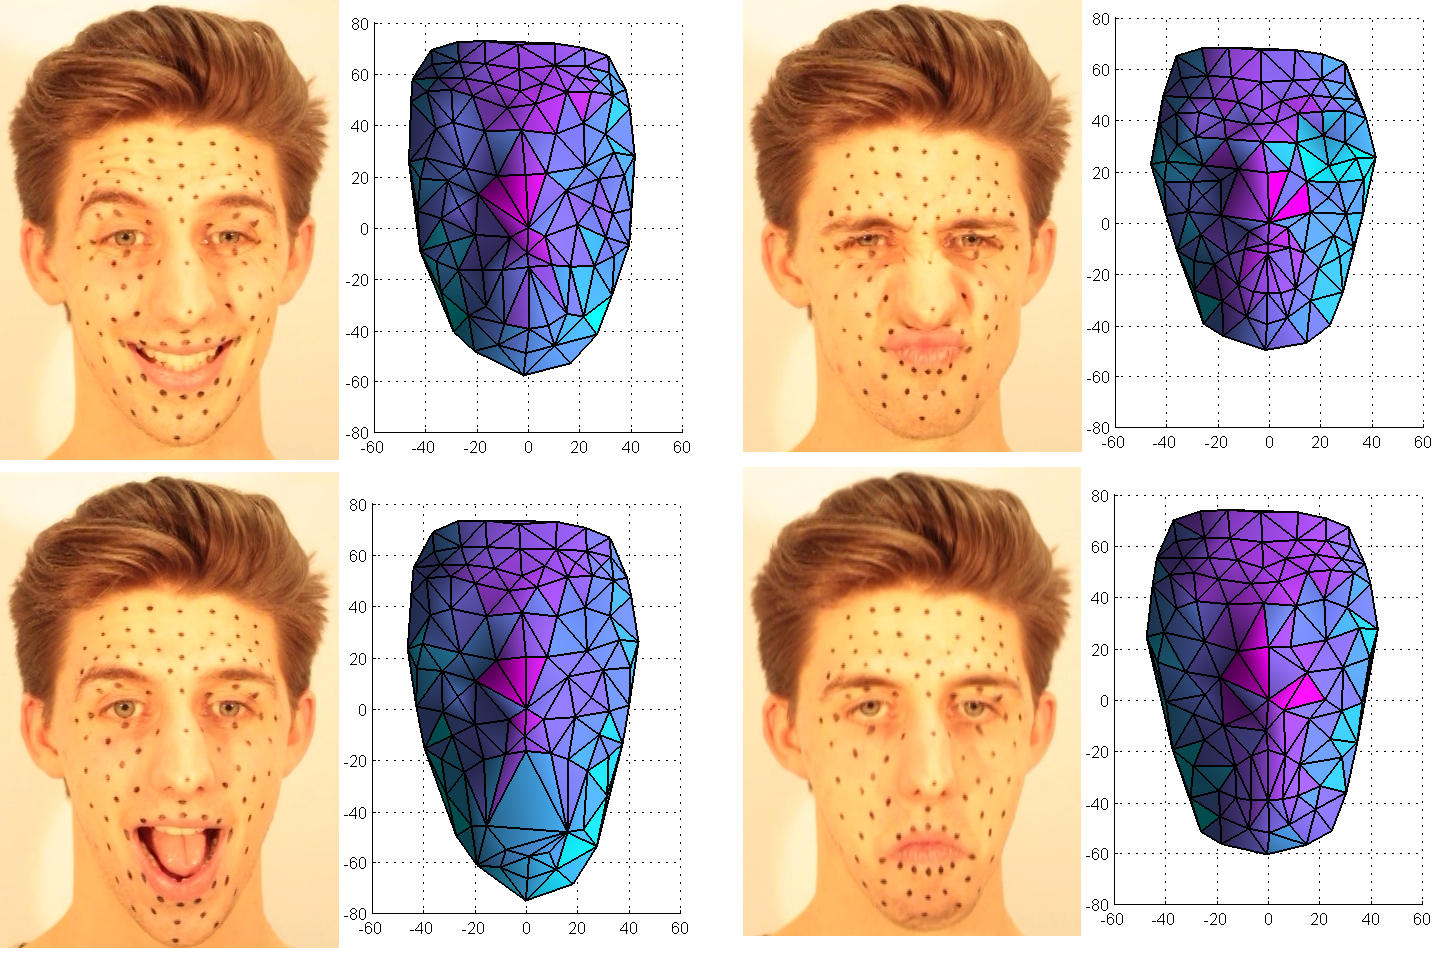
\includegraphics[width=0.7\textwidth]{img/faces}
\caption{\tiny{A sample of reconstructed frames from a captured image sequence.}}
\end{figure}
\end{center}

\end{frame}



\begin{frame}{Head Stabilisation}

\begin{itemize}
\setlength\itemsep{0.5em}
\item We attempt to remove the rigid head motion by performing Procrustes alignment.
\item The head pose in each frame of an image sequence is aligned to the neutral pose. 
\item The 3D point trajectories are also smoothed to remove jittery head motion. 
\end{itemize}

\begin{center}
\begin{figure}
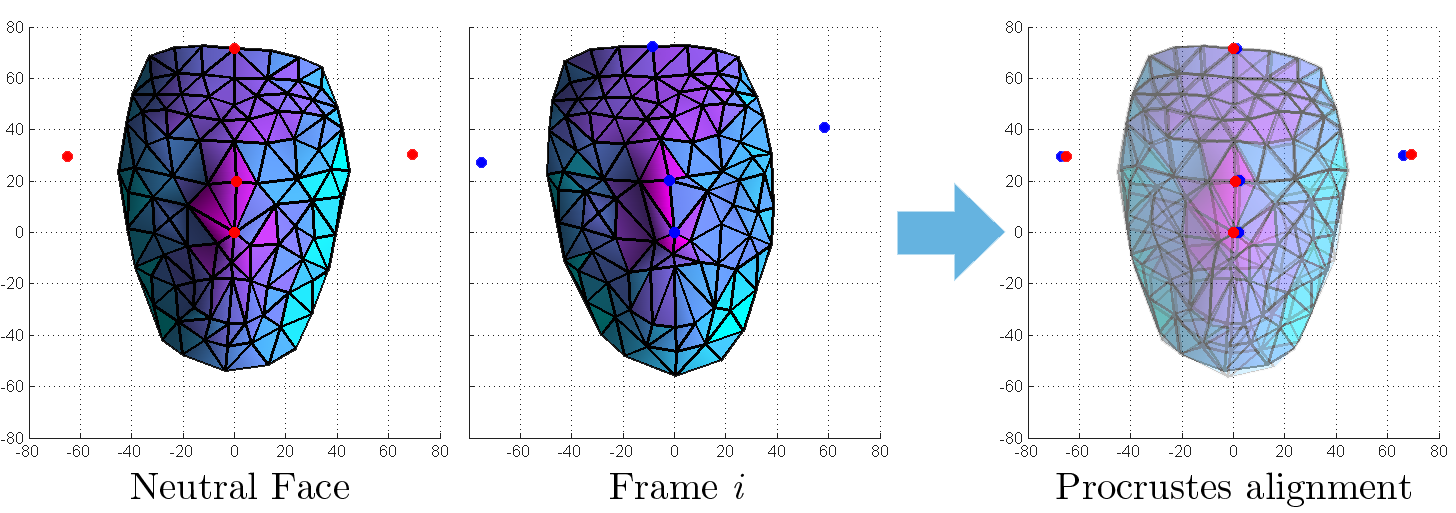
\includegraphics[width=0.8\textwidth]{img/procrustes}
\caption{\tiny{Rigid head motion is removed using Procrustes analysis.}}
\end{figure}
\end{center}

\end{frame}

%----------------------------------------------------------------------
\section{Blendshape Model}
\begin{frame}{General idea}
Given a set of blendshapes $\mathbf{B} = [\bb_1, \ldots, \bb_n]$ and a neutral face $\bb_0$, a new facial expression $\mathbf{F(\w)}$ is a linear combination of the offsets of the basic shapes:
\begin{equation*}
	\underbrace{\F(\w)}_{\text{new expression}} = \underbrace{ \bb_0 }_{\text{neutral face}}+ \sum_{i=1}^N \: \underbrace{w_i}_{\text{weights}} \: \underbrace{|\bb_i - \bb_0|}_{\text{offsets from neutral}}.
\end{equation*}
The \textbf{weights} describe how much each of the basic shapes affect the new expression. 
\end{frame}


\begin{frame}{Designing blendshapes}
\begin{description}
	\item[Option 1] Create blendshapes \textbf{by hand} $\Rightarrow$ correspond to a basic facial expression, for example a raised eyebrow.\\
					$\times$  Hard to produce. \vspace{0.5 cm}
	\item[Option 2] Use \textbf{P}rincipal \textbf{C}omponent \textbf{A}nalysis $\Rightarrow$ automatic construction. \\
					$\times$  Hard to adjust manually.
\end{description}

\end{frame}


\begin{frame}{Estimating weights}
The weights $\w$ are estimating by solving the following:


\begin{minipage}[t]{0.95\linewidth} 
\begin{tcolorbox}[colback=gray!5,colframe=jvagreen, title=Minimisation problem]
\begin{equation*}
	\min_\w \| \underbrace{\hat{\mathbf{B}}}_{\text{matrix with offsets}} \: \: \: \underbrace{\w}_{\text{vector of weights}} - \underbrace{(\F(\w) - \bb_0)}_{\text{offsets of new expression}} \|,
\end{equation*}        
\end{tcolorbox} 
\end{minipage}  \vspace{0.5 cm}

where the weights add up to $1$.

\end{frame}

\begin{frame}{Experiments}
\begin{itemize}
	\item Performance of numerical methods is compared by measuring \textbf{mean squared reconstruction error}.
\begin{figure}
\centering
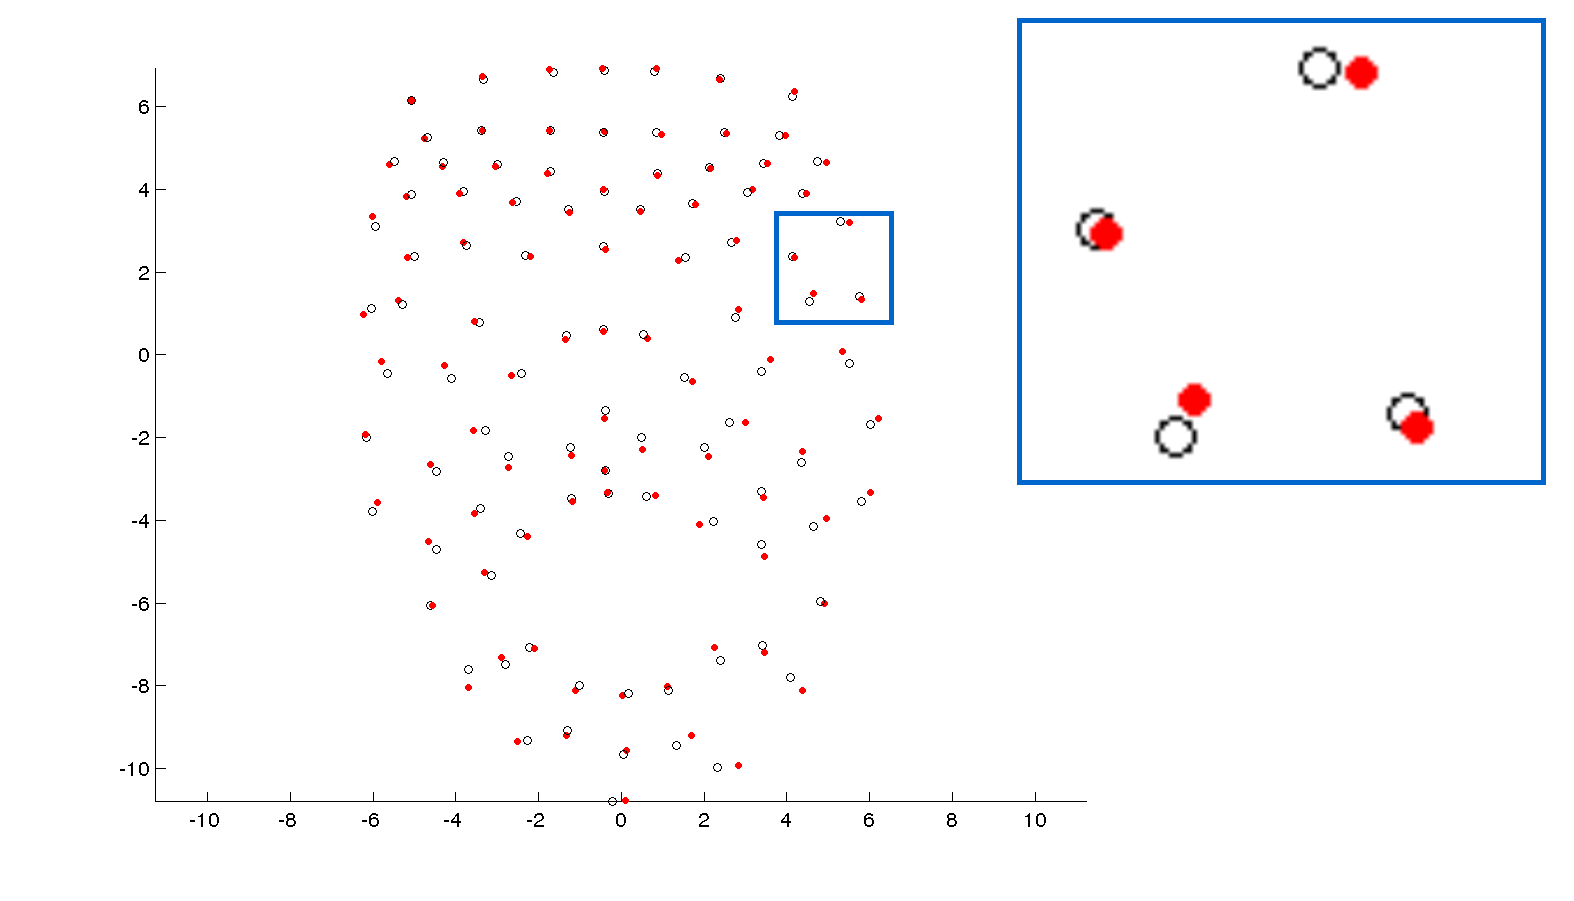
\includegraphics[width=0.4\textwidth]{img/error2}
\end{figure}
	\item Extra shapes.	\begin{figure}[htbp!]
        \centering
        \begin{subfigure}[b]{0.12\textwidth}
                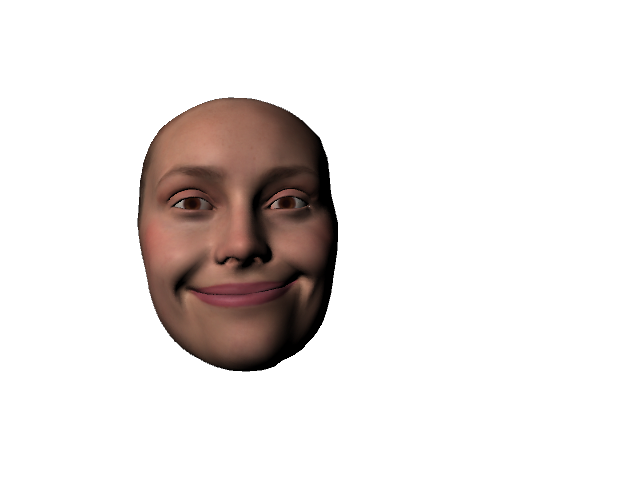
\includegraphics[trim = 50mm 30mm 80mm 30mm,clip,width=\textwidth]{img/lipcorners15.png}
        \end{subfigure}
        ~ %add desired spacing between images, e. g. ~, \quad, \qquad, \hfill etc.
          %(or a blank line to force the subfigure onto a new line)
        \begin{subfigure}[b]{0.12\textwidth}
                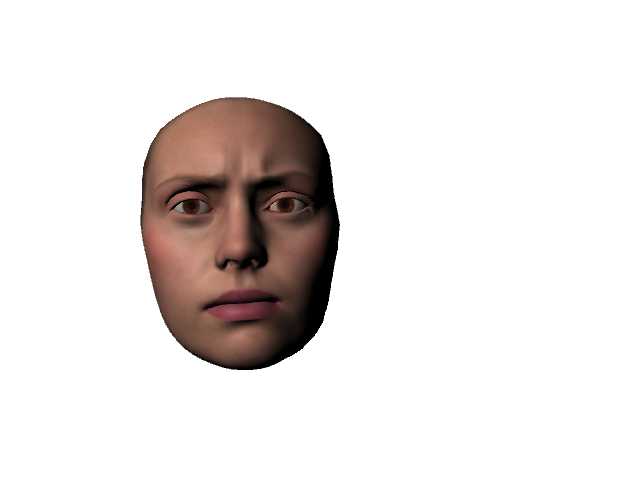
\includegraphics[trim = 50mm 30mm 80mm 30mm,clip,width=\textwidth]{img/eyebrowsin2.png}
        \end{subfigure} ~
        \begin{subfigure}[b]{0.12\textwidth}
                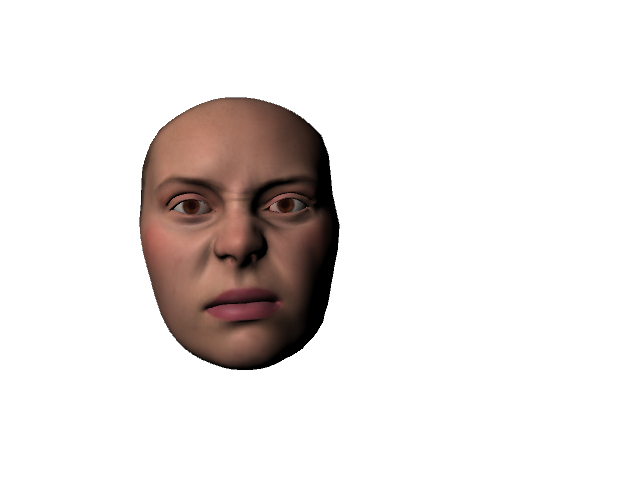
\includegraphics[trim = 50mm 30mm 80mm 30mm,clip,width=\textwidth]{img/nosewrinkle2.png}
        \end{subfigure}
        ~ %add desired spacing between images, e. g. ~, \quad, \qquad, \hfill etc.
          %(or a blank line to force the subfigure onto a new line)
        \begin{subfigure}[b]{0.12\textwidth}
                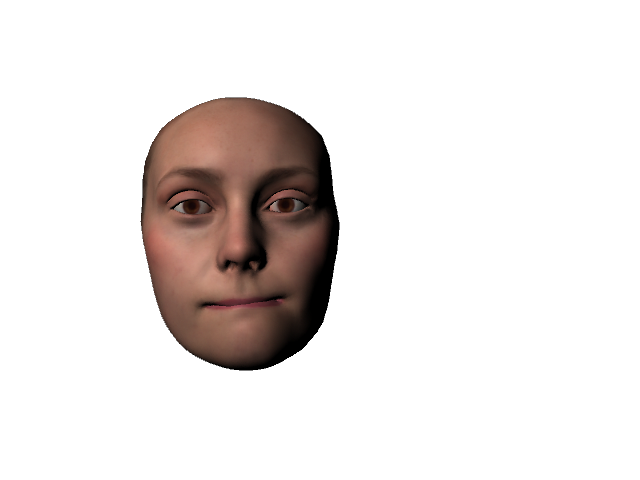
\includegraphics[trim = 50mm 30mm 80mm 30mm,clip,width=\textwidth]{img/mouthsuck.png}
        \end{subfigure}
\end{figure}
\item Different upper bound on each dimension of $\w$.
\end{itemize}

\end{frame}

\begin{frame}{Initial Approach}
\visible<1->{\begin{figure}
        \centering
        \begin{subfigure}[b]{0.43\textwidth}
                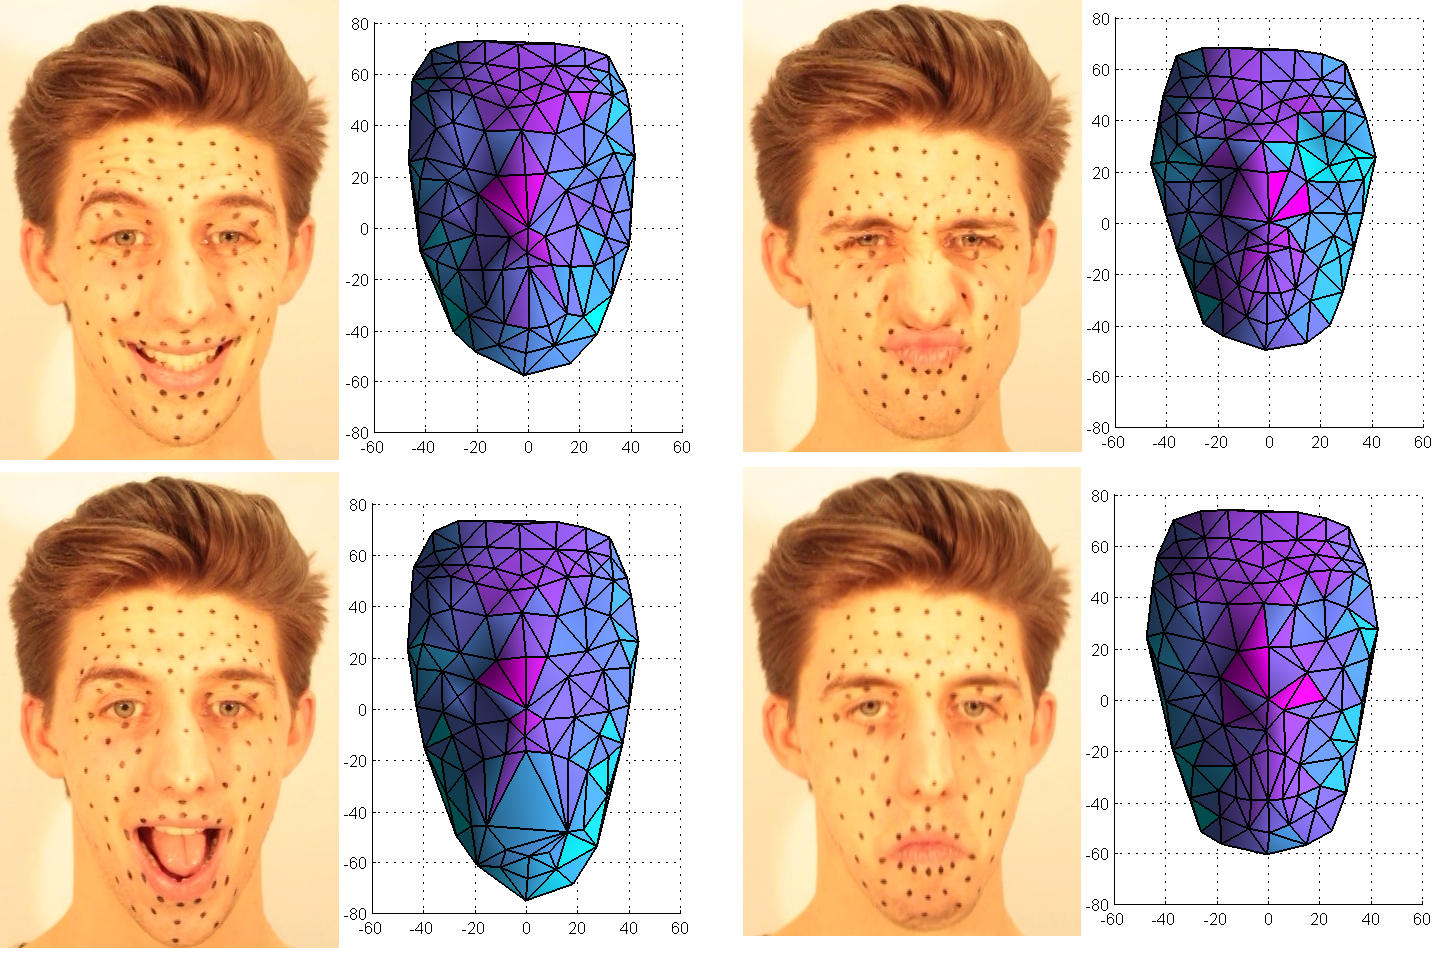
\includegraphics[width=\textwidth]{img/Richdomain}
                \caption{Recorded sequence}
        \end{subfigure}
        \begin{subfigure}[b]{0.2\textwidth}
                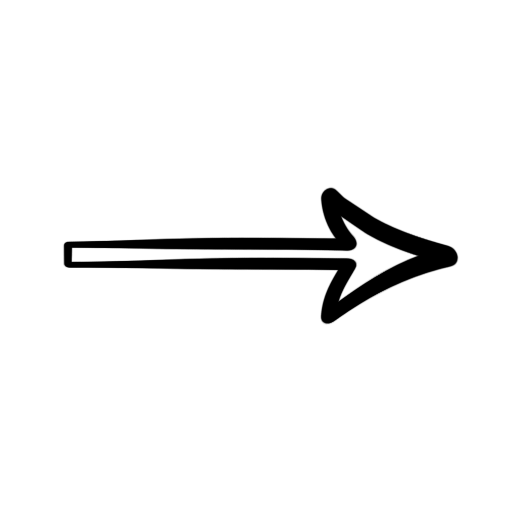
\includegraphics[width=\textwidth]{img/arrow}
                \caption{\hspace{0.2cm} Thin plate splines}
        \end{subfigure}
        \begin{subfigure}[b]{0.3\textwidth}
                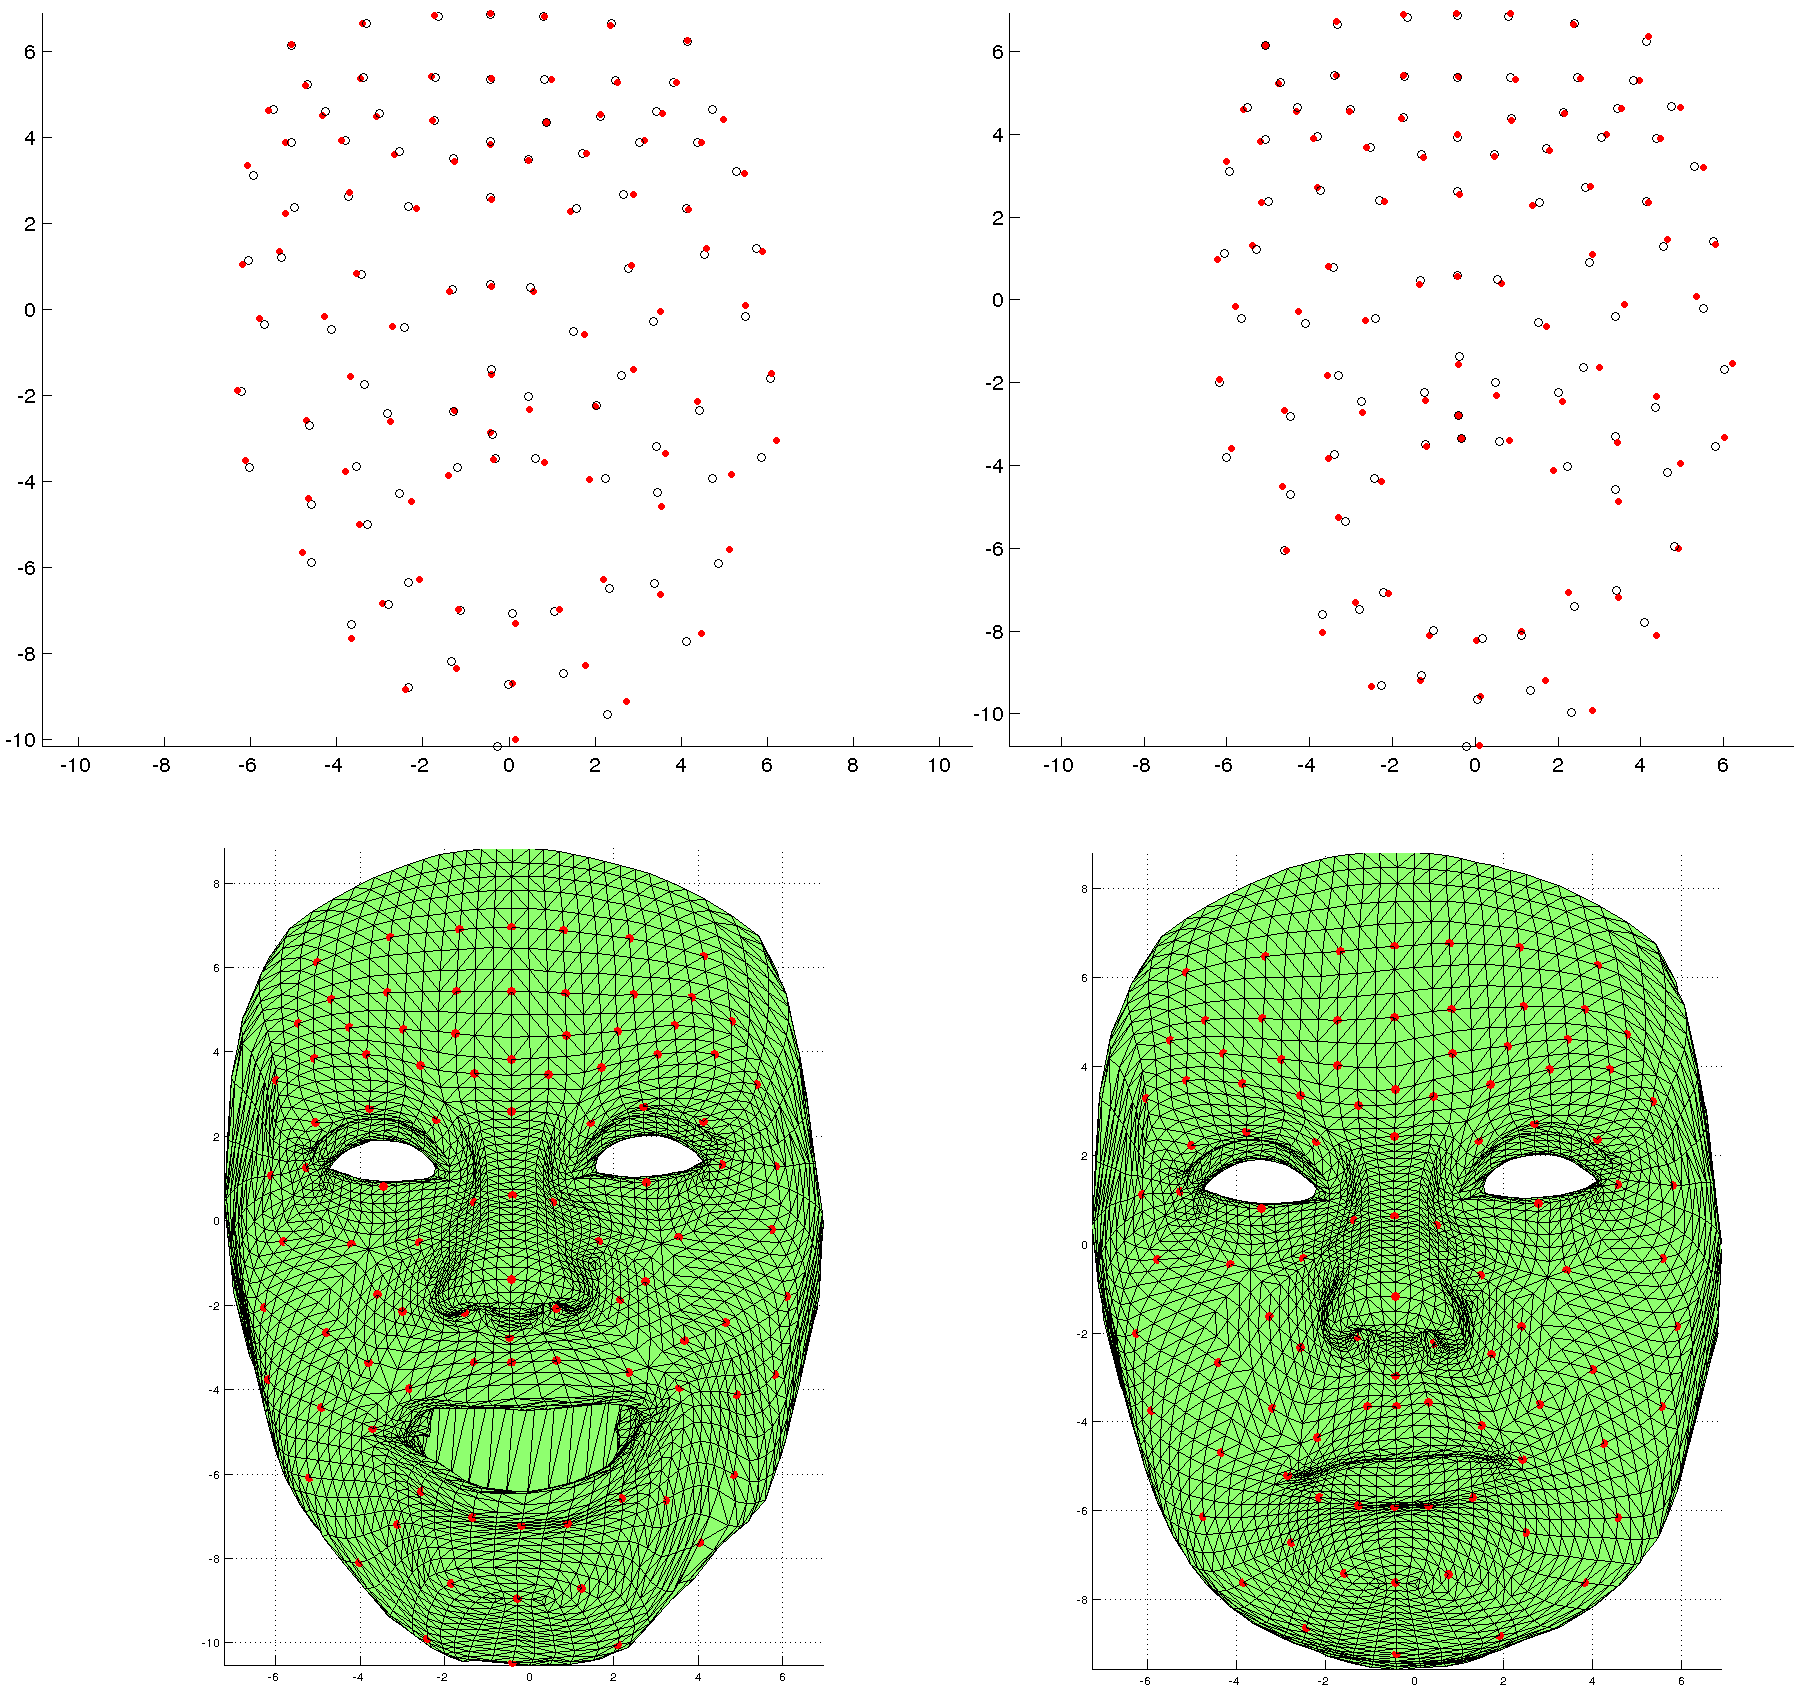
\includegraphics[width=\textwidth]{img/Emilydomain}
                \caption{Emily sequence}
        \end{subfigure}
\end{figure}}

\visible<2->{$\Rightarrow$ Solve for weights in Emily domain.}

\end{frame}

\begin{frame}{Solve for weights in actor's domain}

\visible<1->{\begin{figure}
        \centering
        \begin{subfigure}[b]{0.2\textwidth}
                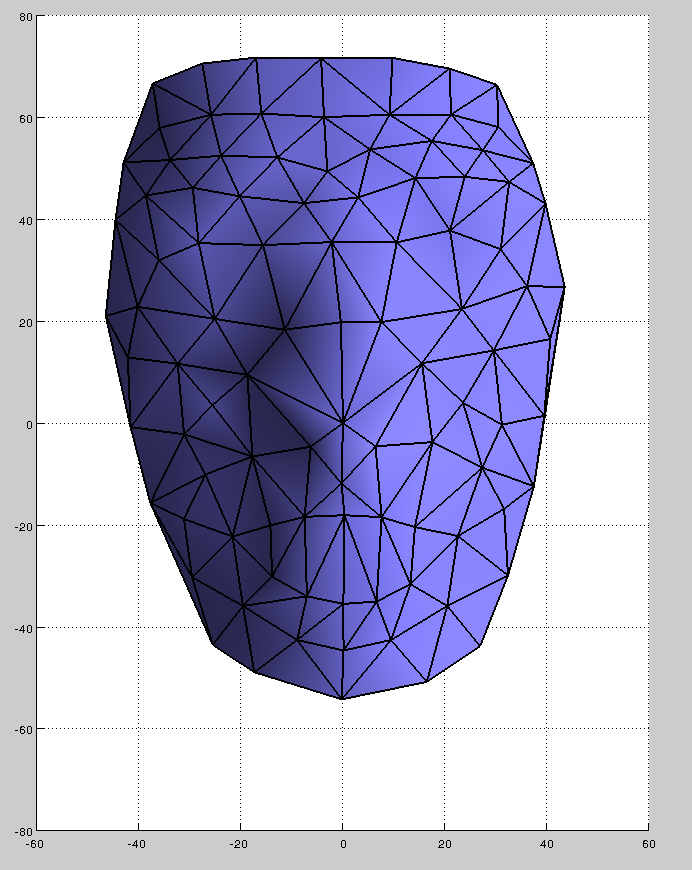
\includegraphics[width=\textwidth]{img/Rneutral}
                \caption{Neutral actor}
        \end{subfigure}
        \begin{subfigure}[b]{0.2\textwidth}
                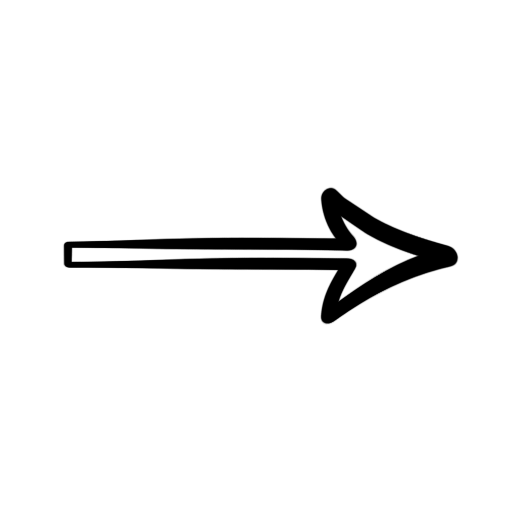
\includegraphics[width=\textwidth]{img/arrow}
                \caption{\hspace{0.2cm} $\mathbf{T}$}
        \end{subfigure}
        \begin{subfigure}[b]{0.3\textwidth}
                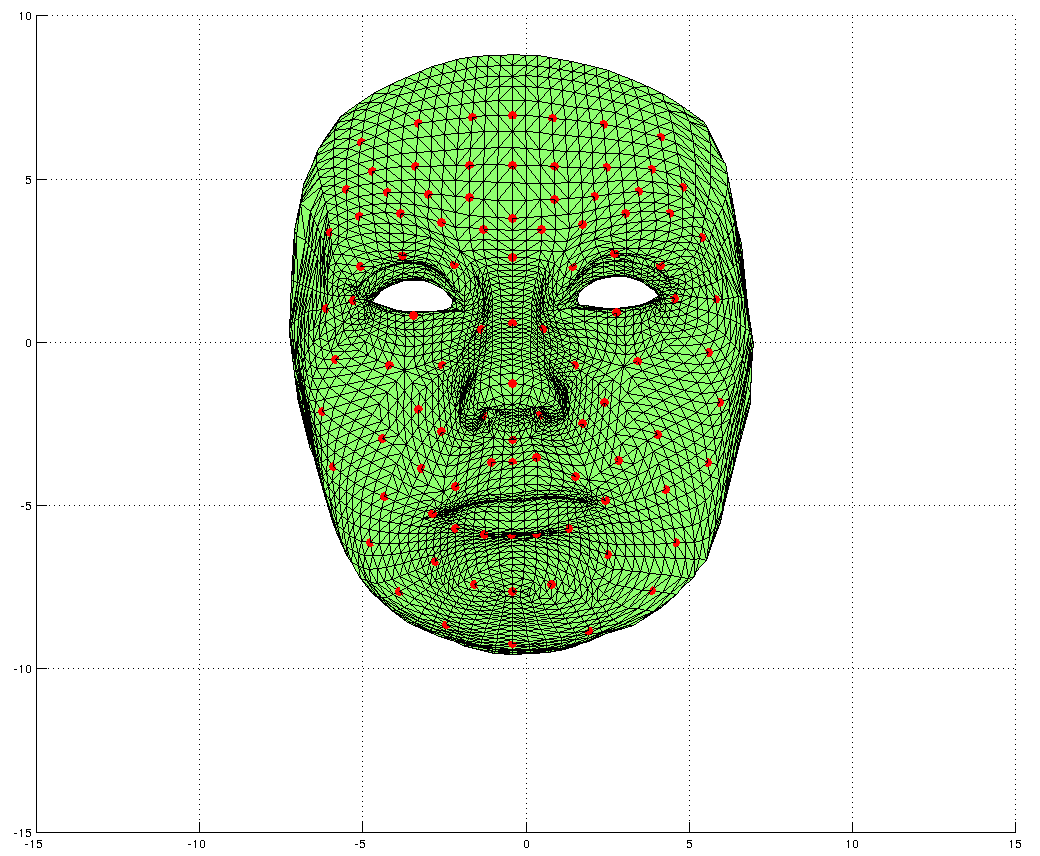
\includegraphics[width=\textwidth]{img/Eneutral}
                \caption{Neutral Emily}
        \end{subfigure}
\end{figure}}

\visible<2->{\begin{figure}
        \centering
        \begin{subfigure}[b]{0.3\textwidth}
                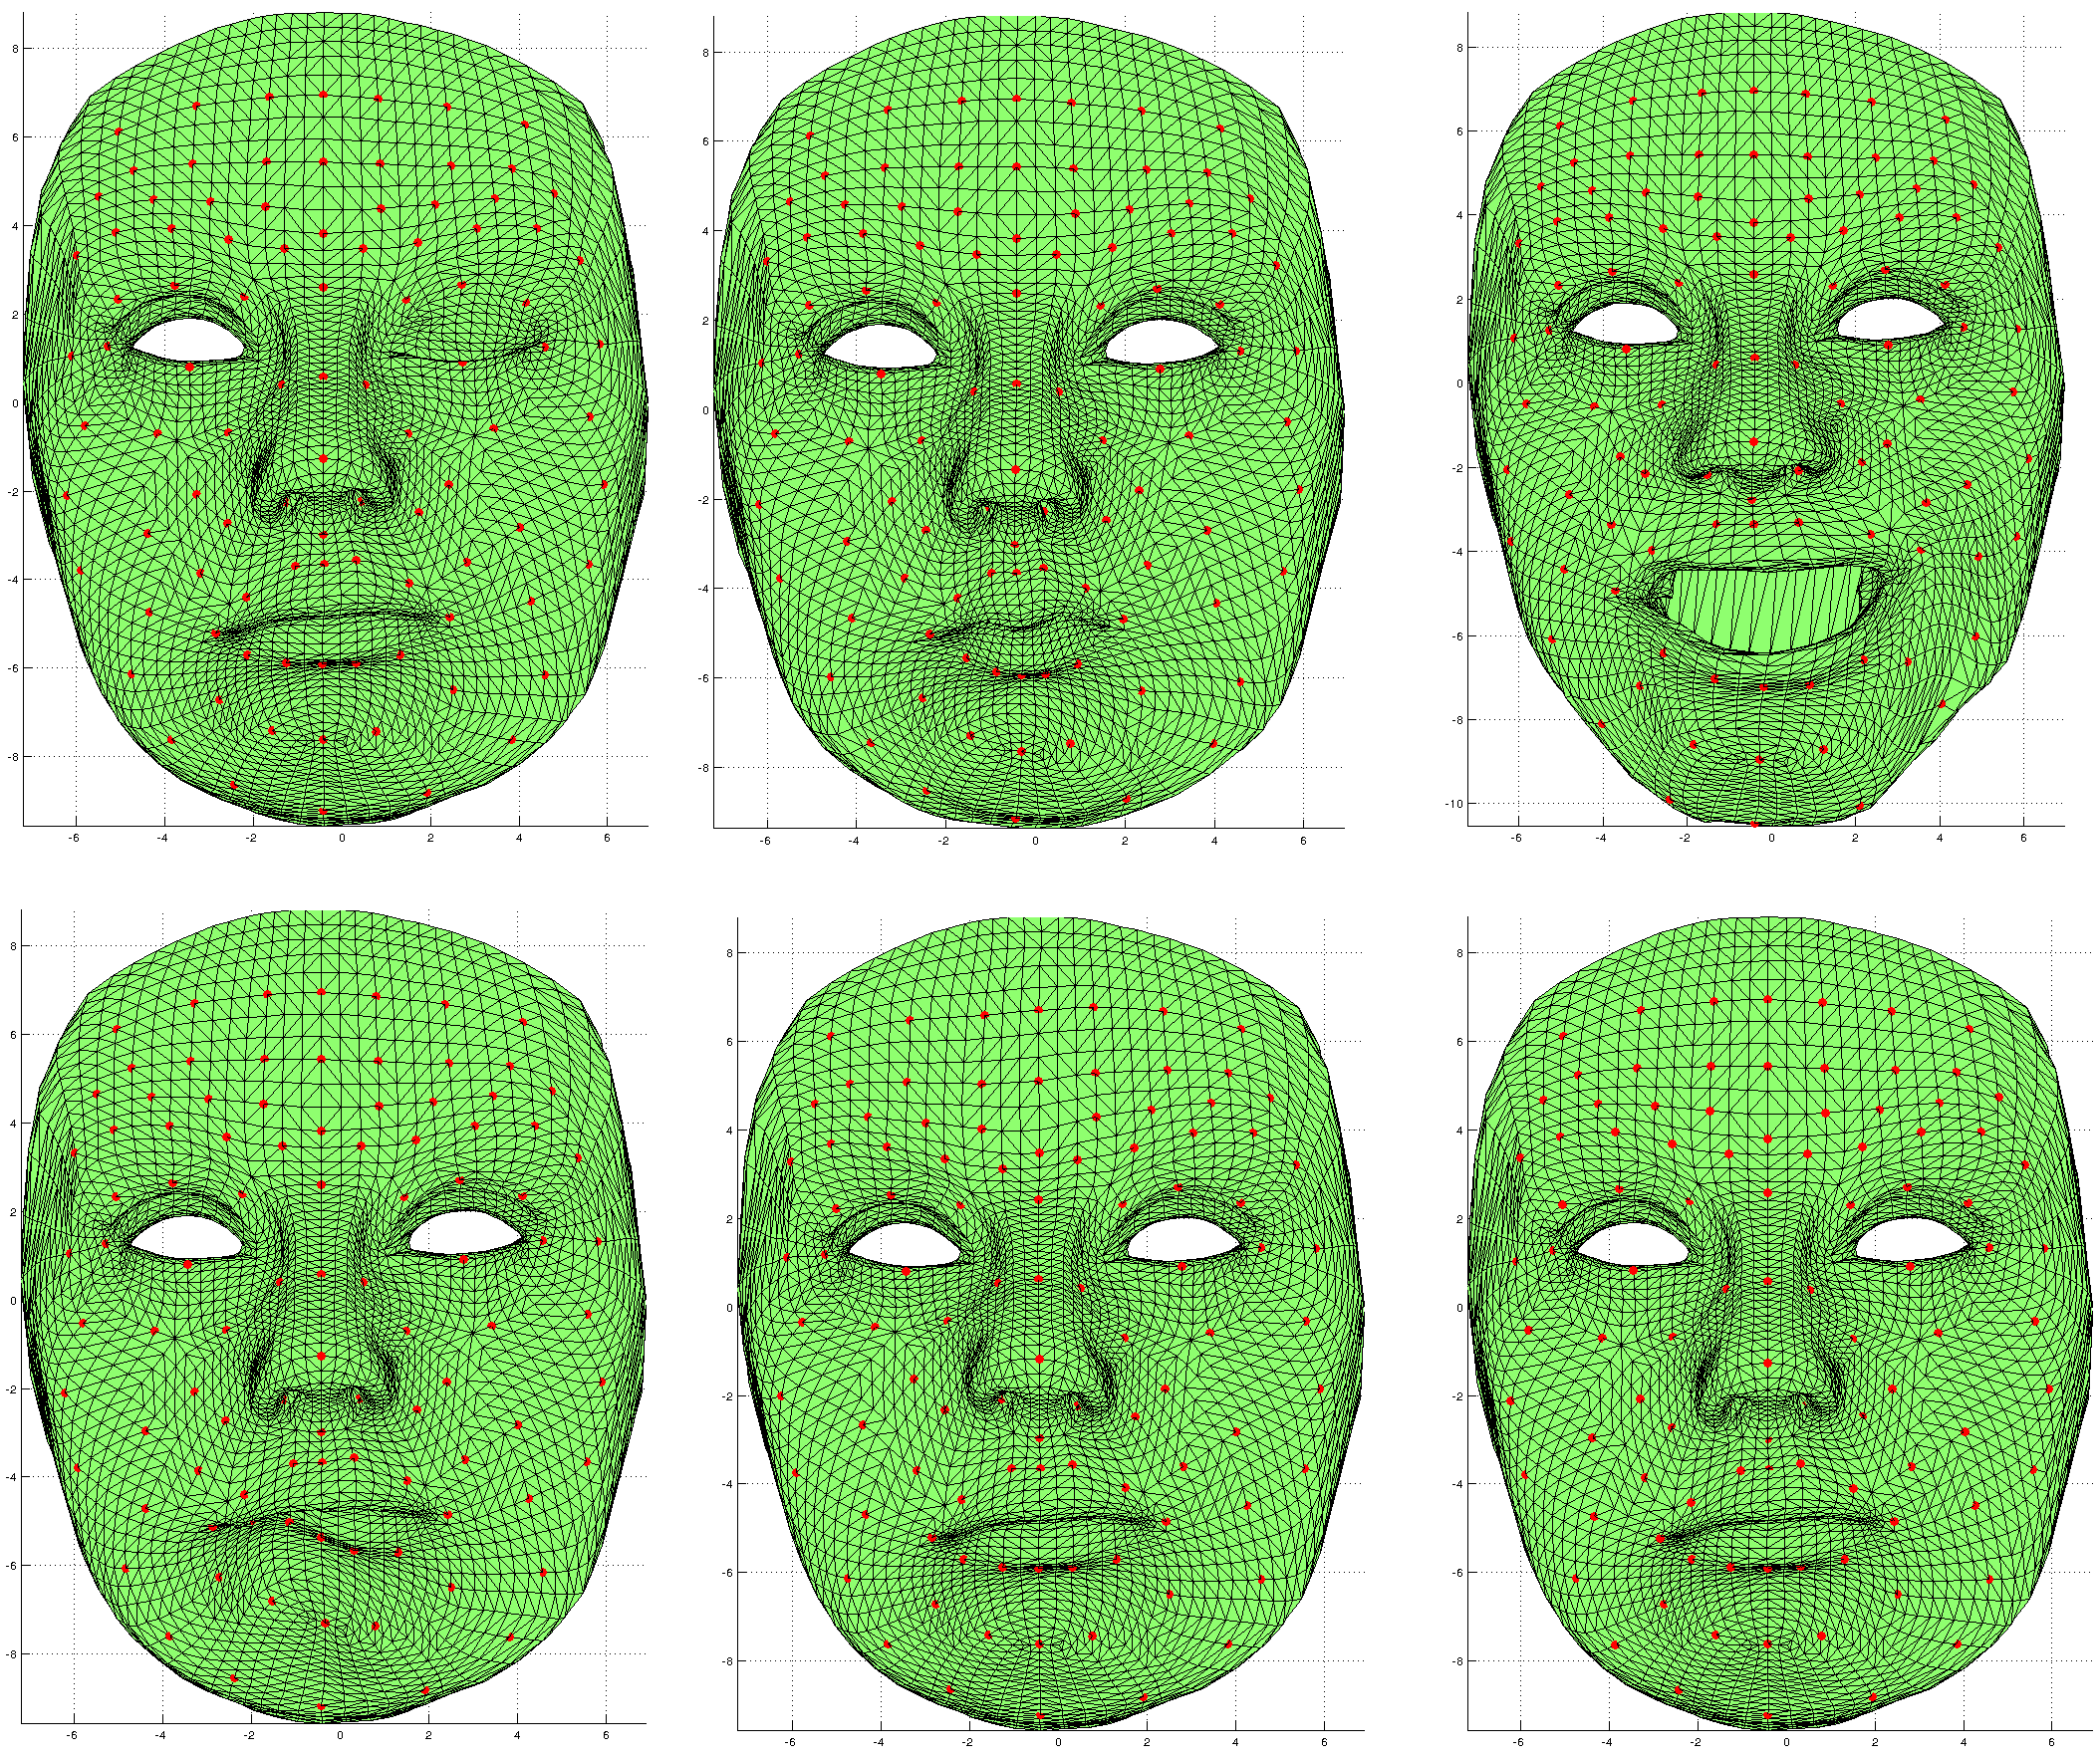
\includegraphics[width=\textwidth]{img/Eblends}
                \caption{Emily blendshapes}
        \end{subfigure}
        \begin{subfigure}[b]{0.2\textwidth}
                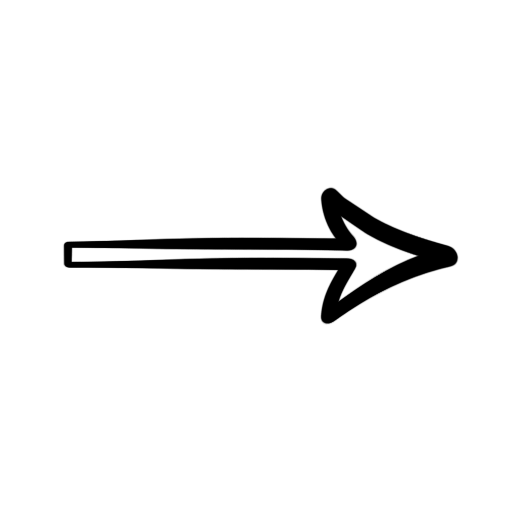
\includegraphics[width=\textwidth]{img/arrow}
                \caption{\hspace{0.2cm} $\mathbf{T}^{-1}$}
        \end{subfigure}
        \begin{subfigure}[b]{0.3\textwidth}
                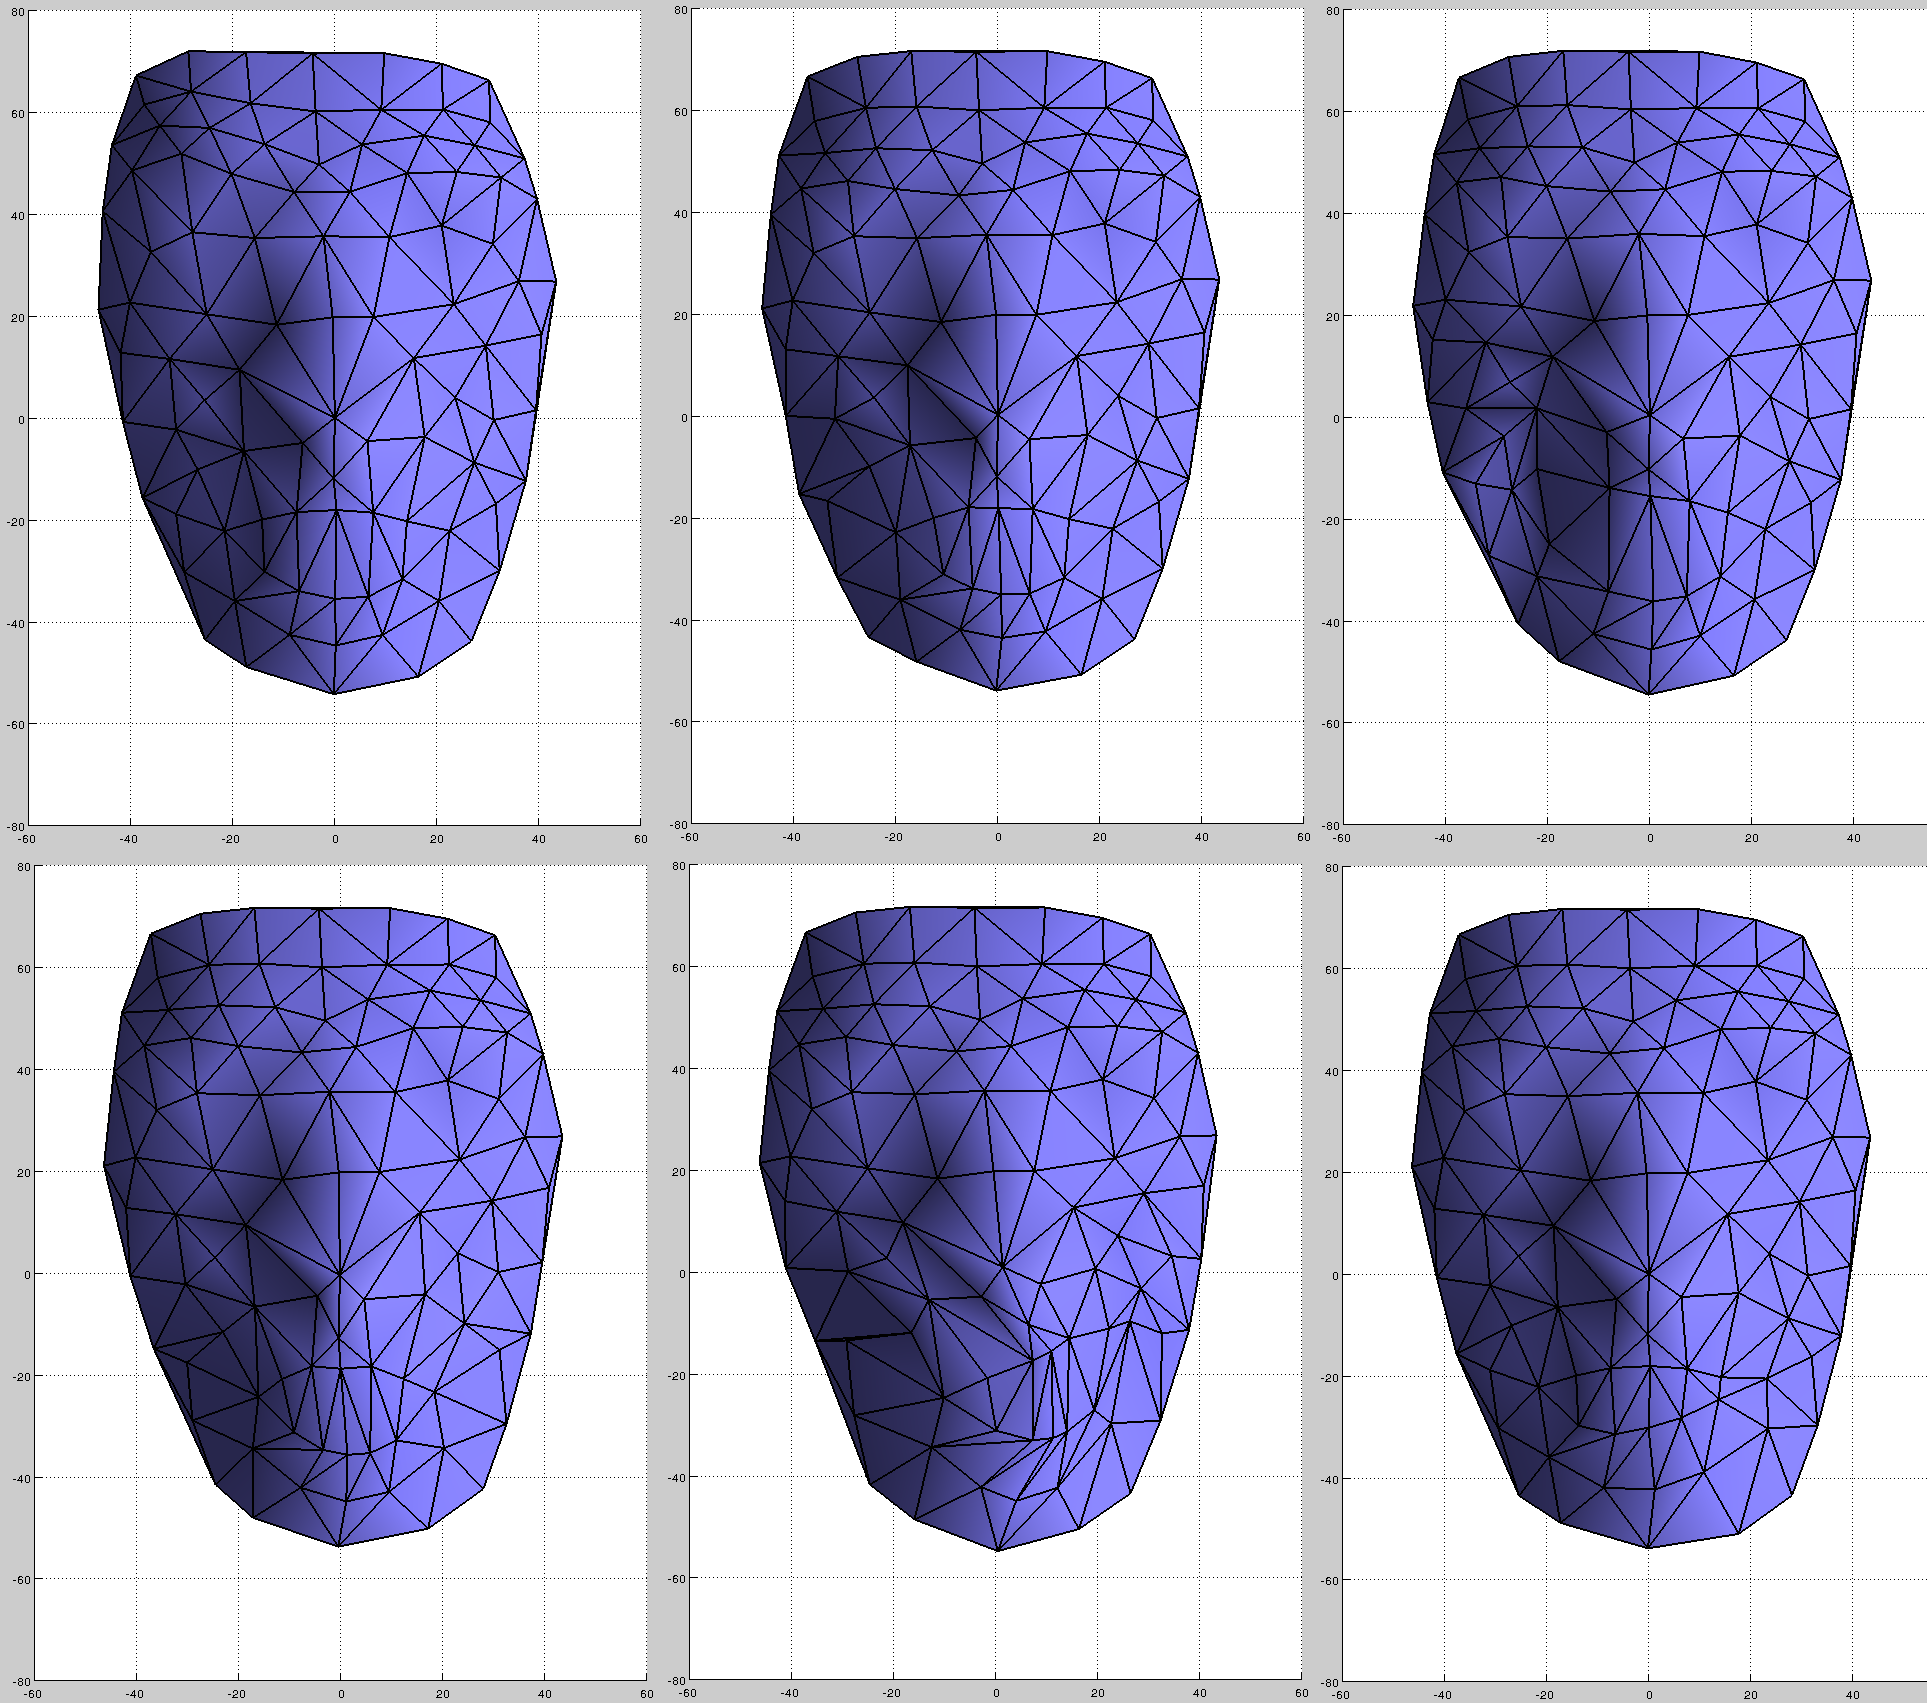
\includegraphics[width=\textwidth]{img/Rblends}
                \caption{Actor's blendshapes}
        \end{subfigure}
\end{figure}}

\end{frame}

\begin{frame}{Issues}
\begin{itemize}
	\item Mismatch of neutral expressions.
	\begin{figure}
        \centering
        \begin{subfigure}[b]{0.2\textwidth}
                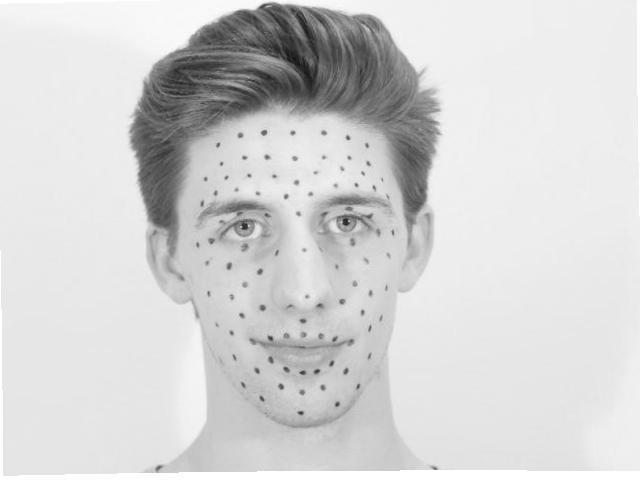
\includegraphics[width=\textwidth]{img/Richard2neutral}
        \end{subfigure}
        \begin{subfigure}[b]{0.2\textwidth}
                \includegraphics[width=\textwidth]{img/Emily2neutral}
        \end{subfigure}
\end{figure}
\end{itemize}

\end{frame}

%----------------------------------------------------------------------
\section{Garoe's Part}
\begin{frame}{Frame name}

\end{frame}


\begin{frame}{Frame name}

\end{frame}


%\begin{center}
%\begin{figure}
%\includegraphics[width=0.5\textwidth]{img/6phongReflexion} ~
%\includegraphics[width=0.5\textwidth]{img/8phongShading}
%\caption*{\tiny{Left shows flat shading, right shows Gouraud shading.}}
%\end{figure}
%\end{center}
%
%\begin{itemize}
%\setlength\itemsep{0.5em}
%\item 
%\end{itemize}

%\begin{multicols}{2}
%\begin{figure}[b!]
%\includegraphics[width=0.4\textwidth]{img/cloth_directions}
%\end{figure}
%
%\vfill
%\columnbreak
%\vspace*{\fill}
%\small{where $F$ are Fresnel terms, $\eta$ are Fresnel coefficients, $g$ is a Gaussian lobe, $k_d$ is a scattering constant, $\gamma$ are Gaussian widths, $\theta_h = (\theta_i+\theta_r)/2$ and $\phi_d = \phi_i-\phi_r$. }
%\end{multicols}


%----------------------------------------------------------------------

\end{document}
